\documentclass[letterpaper,twocolumn,10pt]{article}
\usepackage{usenix}

% to be able to draw some self-contained figs
\usepackage{tikz}
\usepackage{amsmath}
\usepackage{amsfonts}
\usepackage[labelfont=bf]{caption}

% inlined bib file
\usepackage{filecontents}

%-------------------------------------------------------------------------------
\begin{filecontents}{\jobname.bib}
%-------------------------------------------------------------------------------
@inproceedings {ULEvsCFS,
  author = {Justinien Bouron and Sebastien Chevalley and Baptiste Lepers and Willy Zwaenepoel and Redha Gouicem and Julia Lawall and Gilles Muller and Julien Sopena},
  title = {The Battle of the Schedulers: {FreeBSD} {ULE} vs. Linux {CFS}},
  booktitle = {2018 USENIX Annual Technical Conference (USENIX ATC 18)},
  year = {2018},
  isbn = {978-1-931971-44-7},
  address = {Boston, MA},
  pages = {85--96},
  url = {https://www.usenix.org/conference/atc18/presentation/bouron},
  publisher = {USENIX Association},
  month = jul
}

@inproceedings{mlfq,
  author = {Corbat{\'o}, Fernando J. and Merwin-Daggett, Marjorie and Daley, Robert C.},
  title = {An experimental time-sharing system},
  year = {1962},
  isbn = {9781450378758},
  publisher = {Association for Computing Machinery},
  address = {New York, NY, USA},
  url = {https://doi.org/10.1145/1460833.1460871},
  doi = {10.1145/1460833.1460871},
  abstract = {It is the purpose of this paper to discuss briefly the need for time-sharing, some of the implementation problems, an experimental timesharing system which has been developed for the contemporary IBM 7090, and finally a scheduling algorithm of one of us (FJC) that illustrates some of the techniques which may be employed to enhance and be analyzed for the performance limits of such a time-sharing system.},
  booktitle = {Proceedings of the May 1-3, 1962, Spring Joint Computer Conference},
  pages = {335–344},
  numpages = {10},
  location = {San Francisco, California},
  series = {AIEE-IRE '62 (Spring)}
}

@inproceedings{DRR,
  author = {Shreedhar, M. and Varghese, George},
  title = {Efficient fair queueing using deficit round robin},
  year = {1995},
  isbn = {0897917111},
  publisher = {Association for Computing Machinery},
  address = {New York, NY, USA},
  url = {https://doi.org/10.1145/217382.217453},
  doi = {10.1145/217382.217453},
  abstract = {Fair queuing is a technique that allows each flow passing through a network device to have a fair share of network resources. Previous schemes for fair queuing that achieved nearly perfect fairness were expensive to implement: specifically, the work required to process a packet in these schemes was O(log(n)), where n is the number of active flows. This is expensive at high speeds. On the other hand, cheaper approximations of fair queuing that have been reported in the literature exhibit unfair behavior. In this paper, we describe a new approximation of fair queuing, that we call Deficit Round Robin. Our scheme achieves nearly perfect fairness in terms of throughput, requires only O(1) work to process a packet, and is simple enough to implement in hardware. Deficit Round Robin is also applicable to other scheduling problems where servicing cannot be broken up into smaller units, and to distributed queues.},
  booktitle = {Proceedings of the Conference on Applications, Technologies, Architectures, and Protocols for Computer Communication},
  pages = {231–242},
  numpages = {12},
  location = {Cambridge, Massachusetts, USA},
  series = {SIGCOMM '95}
}

@misc{sysbench,
  author = {Alexey Kopytov},
  title = {sysbench: Scriptable database and system performance benchmark},
  howpublished = {\url{https://github.com/akopytov/sysbench}},
  note = {GitHub repository}
}
\end{filecontents}

\usetikzlibrary{matrix, positioning, calc, arrows.meta}

%-------------------------------------------------------------------------------
\begin{document}
%-------------------------------------------------------------------------------

%don't want date printed
\date{}

% make title bold and 14 pt font (Latex default is non-bold, 16 pt)
\title{\Large \bf Progress Report: Grid, A Multi-dimensional MLFQ Scheduler}

%for single author (just remove % characters)
\author{
{\rm Jeffrey Jiang}\\
Stony Brook University
} % end author

\maketitle

%-------------------------------------------------------------------------------
\section{Grid Scheduler Current Design}
%-------------------------------------------------------------------------------

My proposed scheduler, called the grid scheduler, is based on the multilevel feedback 
queue (MLFQ) scheduling~\cite{mlfq} like FreeBSD's ULE except modifications were made 
to treat the latency requirement and the ideal time slice length orthogonally.
Several design changes have been made since the proposal including a mechanism 
to guarantee fairness. 

\subsection{Data Structure}

The grid scheduler will use a per-cpu two-dimensional grid of feedback dispatch queues. 
Figure~\ref{fig:mlfq_grid} shows the structure of the scheduler I am proposing. 
The grid is \(8\times 8\), and each cell is a queue. The x-axis of the grid represent 
the time slice length assigned processes within queues of that column, and the y-axis 
represents the latency requirement of the process. Together, if a process is in the 
dispatch queue at row \(i\) and column \(j\), then it has the latency requirement assigned to 
row \(i\) and the time slice at column \(j\). The \(8\times 8\) grid was chosen, so 
there is a total of \(64\) queues. This allows a summary of the grid represented as a 
bitmap in a \(64\)-bit integer called a summary which allows us to use bitwise 
operations to quickly query the state of these queues.

\begin{figure}
  \begin{center}
    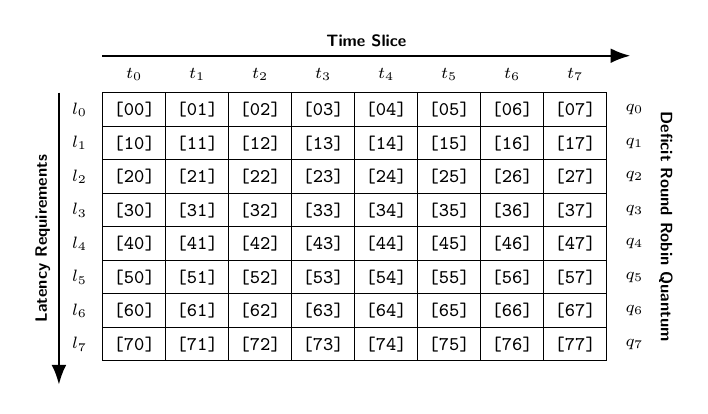
\begin{tikzpicture}[
    scale=0.85, transform shape, % Scales down the entire diagram
    queue node/.style={draw, minimum width=0.6cm, minimum height=0.4cm, anchor=center, font=\scriptsize\ttfamily},
    axis arrow/.style={-{Latex[length=2.5mm]}, thick},
    grid node/.style={draw, minimum width=0.8cm, minimum height=0.4cm, anchor=center, font=\scriptsize\ttfamily}
]
    % Define the grid
    \matrix (mat) [
        matrix of nodes,
        nodes={grid node},
        column sep=-\pgflinewidth,
        row sep=-\pgflinewidth,
        nodes in empty cells=false
    ] {
        |[name=m00]| [00] & |[name=m01]| [01] & |[name=m02]| [02] & |[name=m03]| [03] & |[name=m04]| [04] & |[name=m05]| [05] & |[name=m06]| [06] & |[name=m07]| [07] \\
        |[name=m10]| [10] & |[name=m11]| [11] & |[name=m12]| [12] & |[name=m13]| [13] & |[name=m14]| [14] & |[name=m15]| [15] & |[name=m16]| [16] & |[name=m17]| [17] \\
        |[name=m20]| [20] & |[name=m21]| [21] & |[name=m22]| [22] & |[name=m23]| [23] & |[name=m24]| [24] & |[name=m25]| [25] & |[name=m26]| [26] & |[name=m27]| [27] \\
        |[name=m30]| [30] & |[name=m31]| [31] & |[name=m32]| [32] & |[name=m33]| [33] & |[name=m34]| [34] & |[name=m35]| [35] & |[name=m36]| [36] & |[name=m37]| [37] \\
        |[name=m40]| [40] & |[name=m41]| [41] & |[name=m42]| [42] & |[name=m43]| [43] & |[name=m44]| [44] & |[name=m45]| [45] & |[name=m46]| [46] & |[name=m47]| [47] \\
        |[name=m50]| [50] & |[name=m51]| [51] & |[name=m52]| [52] & |[name=m53]| [53] & |[name=m54]| [54] & |[name=m55]| [55] & |[name=m56]| [56] & |[name=m57]| [57] \\
        |[name=m60]| [60] & |[name=m61]| [61] & |[name=m62]| [62] & |[name=m63]| [63] & |[name=m64]| [64] & |[name=m65]| [65] & |[name=m66]| [66] & |[name=m67]| [67] \\
        |[name=m70]| [70] & |[name=m71]| [71] & |[name=m72]| [72] & |[name=m73]| [73] & |[name=m74]| [74] & |[name=m75]| [75] & |[name=m76]| [76] & |[name=m77]| [77] \\
    };

    % X-axis labels (Quanta) - Moved to top
    \node [above=0.05cm of m00, font=\scriptsize\ttfamily] {$t_0$};
    \node [above=0.05cm of m01, font=\scriptsize\ttfamily] {$t_1$};
    \node [above=0.05cm of m02, font=\scriptsize\ttfamily] {$t_2$};
    \node [above=0.05cm of m03, font=\scriptsize\ttfamily] {$t_3$};
    \node [above=0.05cm of m04, font=\scriptsize\ttfamily] {$t_4$};
    \node [above=0.05cm of m05, font=\scriptsize\ttfamily] {$t_5$};
    \node [above=0.05cm of m06, font=\scriptsize\ttfamily] {$t_6$};
    \node [above=0.05cm of m07, font=\scriptsize\ttfamily] {$t_7$};
    
    % Quanta Arrow - Moved to top
    \draw[axis arrow] ([xshift=0.15cm, yshift=0.4cm]mat.north west) -- ([xshift=0.2cm, yshift=0.4cm]mat.north east) node[midway, above, font=\sffamily\bfseries\scriptsize] {Time Slice};

    % Y-axis labels (Latency)
    \node [left=0.1cm of m00, font=\scriptsize\ttfamily] {$l_0$};
    \node [left=0.1cm of m10, font=\scriptsize\ttfamily] {$l_1$};
    \node [left=0.1cm of m20, font=\scriptsize\ttfamily] {$l_2$};
    \node [left=0.1cm of m30, font=\scriptsize\ttfamily] {$l_3$};
    \node [left=0.1cm of m40, font=\scriptsize\ttfamily] {$l_4$};
    \node [left=0.1cm of m50, font=\scriptsize\ttfamily] {$l_5$};
    \node [left=0.1cm of m60, font=\scriptsize\ttfamily] {$l_6$};
    \node [left=0.1cm of m70, font=\scriptsize\ttfamily] {$l_7$};
    
    % Latency Arrow
    \draw[axis arrow] ([xshift=-0.5cm, yshift=-0.15cm]mat.north west) -- ([xshift=-0.5cm, yshift=-0.2cm]mat.south west) node[midway, above, rotate=90, font=\sffamily\bfseries\scriptsize] {Latency Requirements};

    % Quanta for Deficit Round Robin
    \node [right=0.15cm of m07, font=\scriptsize\ttfamily] {$q_0$};
    \node [right=0.15cm of m17, font=\scriptsize\ttfamily] {$q_1$};
    \node [right=0.15cm of m27, font=\scriptsize\ttfamily] {$q_2$};
    \node [right=0.15cm of m37, font=\scriptsize\ttfamily] {$q_3$};
    \node [right=0.15cm of m47, font=\scriptsize\ttfamily] {$q_4$};
    \node [right=0.15cm of m57, font=\scriptsize\ttfamily] {$q_5$};
    \node [right=0.15cm of m67, font=\scriptsize\ttfamily] {$q_6$};
    \node [right=0.15cm of m77, font=\scriptsize\ttfamily] {$q_7$};

    % DRR Quanta Label
    \draw[axis arrow, draw=none] ([xshift=0.5cm, yshift=0cm]mat.north east) -- ([xshift=0.5cm, yshift=0cm]mat.south east) node[midway, above, rotate=-90, font=\sffamily\bfseries\scriptsize] {Deficit Round Robin Quantum};

\end{tikzpicture}
  \end{center}
  \captionsetup{font=scriptsize}
  \vspace{-10pt}
  \caption{\scriptsize\label{fig:mlfq_grid} The scheduler is arranged in a 
  two-dimensional grid. Each cell of the grid is a eBPF dispatch queue.
  Given \(i\) and \(j\) is the row and column respectively, the parameters 
  \(t_j\), \(l_i\), and \(q_i\) can be configured in user-space when
  launching the scheduler.}
\end{figure}

\subsection{Scheduling Policy}

Similar to MLFQ, the scheduler will adaptively move processes between different
queues with the goal to find the ideal queue which best suits the process'
behavior. Because of the grid structure, this involves determining the time
slice length and the latency requirement of the process dynamically. The
policies that dictates how a process moves between cells of the grid scheduler
is described below:

\subsubsection{Time Slice Length Policy}\label{sec:timeslice}

Let \(T\) be the time a process spends running and \(t_c\) be the allotted 
time slice the scheduler gives which corresponds to time slice configured
for column \(c\) of the grid. If \(T\ge t_c\), then the next column assigned
to this task is \(\min(c+1,\text{NR\_COLS}-1)\) where \(\text{NR\_COLS}\) is
the total number of columns in the grid. If \(T < t_c/2\), then the next
column for this task is \(\max(c-1,0)\).

\subsubsection{Latency Requirement Policy}\label{sec:latency}

In the initial proposal, latency requirement was going to be determined from
examining the wake queue that a process wakes from. However, the grid scheduler
will use a simpler design which leverages eBPF.\@ The scheduler will install 
additional eBPF handlers to system call such as \texttt{sys\_futex}, 
\texttt{sys\_read}, etc.\ to examine why a process is no longer runnable. These
handlers will simply set a flag describing the system call that was invoked.
This flag will be read by the scheduler when determining the latency requirement.
This should offer flexibility and may even allow the a user to specify the priorities 
based the system call involved.

\subsubsection{Dispatching and Fairness}\label{sec:dispatching}

The policy decisions on what row and column of the grid to place a runnable task
is computed when the task gets preempted and is no longer running on the CPU.\@
The row and column is stored until the task is runnable again. When the task
is runnable, the task is inserted into the dispatch queue corresponding to this
row and column of the grid belonging to the current CPU.\@ Importantly, CPU
assignment and grid position are decoupled to allow the native load balancer
to move tasks around freely.

Once the task is on the dispatch queue, it may be scheduled to run on a CPU by a
scheduler. The scheduler gives priority to rows with a lower latency requirement.
When a task wakes up, its latency requirement is retrieved. If the running task's
remaining time slice exceeds this latency requirement, the running task is
preempted. This helps the scheduler satisfy the latency requirements of tasks.

However, due to eBPF's restriction that runnable processes on a dispatch queue must run
on a CPU within 30 seconds, the grid scheduler must ensure fairness. The proposal's
design suggested using the deficit round robin (DRR) algorithm to ensure 
fairness~\cite{DRR}. The current design implements DRR, but at grid row granularity. 
This ensures fairness between tasks with different latency requirement. To ensure
fairness within a row of the grid, a standard round robin is performed between
the queues of the row. This should ensure fairness and avoid potential starvation
of a task.

\subsubsection{Load Balancing}

The load balancing that grid will use is currently simple. The goal of the
load balancer will be to evenly distribute the number of tasks between all the
cores. This will be done by careful placement of the tasks on queues belonging
to other CPUs with low loads. Additionally, CPUs which fail to schedule a task
from their own grid are responsible for stealing a task from another as well.

%-------------------------------------------------------------------------------
\section{Implementation Progress}
%-------------------------------------------------------------------------------

I have begun implementing the scheduler in eBPF.\@ I have successfully set up
my development environment and build system that will allow me to rapidly
iterate my development. 

I have implemented the user-space application that will launch my grid scheduler 
using \texttt{libbpf} and helpers functions provided by \texttt{scx}. This
user-space application is also responsible for passing configuration parameters
to the scheduler. There are three main configuration parameters that can be
specified through the command line arguments: (1) target latency for each row;
(2) time slice length of each column; and (3) the deficit round robin quantum
for each row. 

For the scheduler itself, I have written a preliminary implementation. This
implementation creates the per-CPU dispatch queues, enqueues tasks onto these
queues, and dispatches tasks on the queues based on the algorithms described in
Section~\ref{sec:dispatching}. The load balancing has not been implemented.
In addition, while the time slice length policy described in 
Section~\ref{sec:timeslice} has been implemented, the latency requirement 
policy described in Section~\ref{sec:latency} has not. Figure~\ref{fig:logs}
shows some debug logs from the grid scheduler.

\begin{figure}
  \begin{center}
    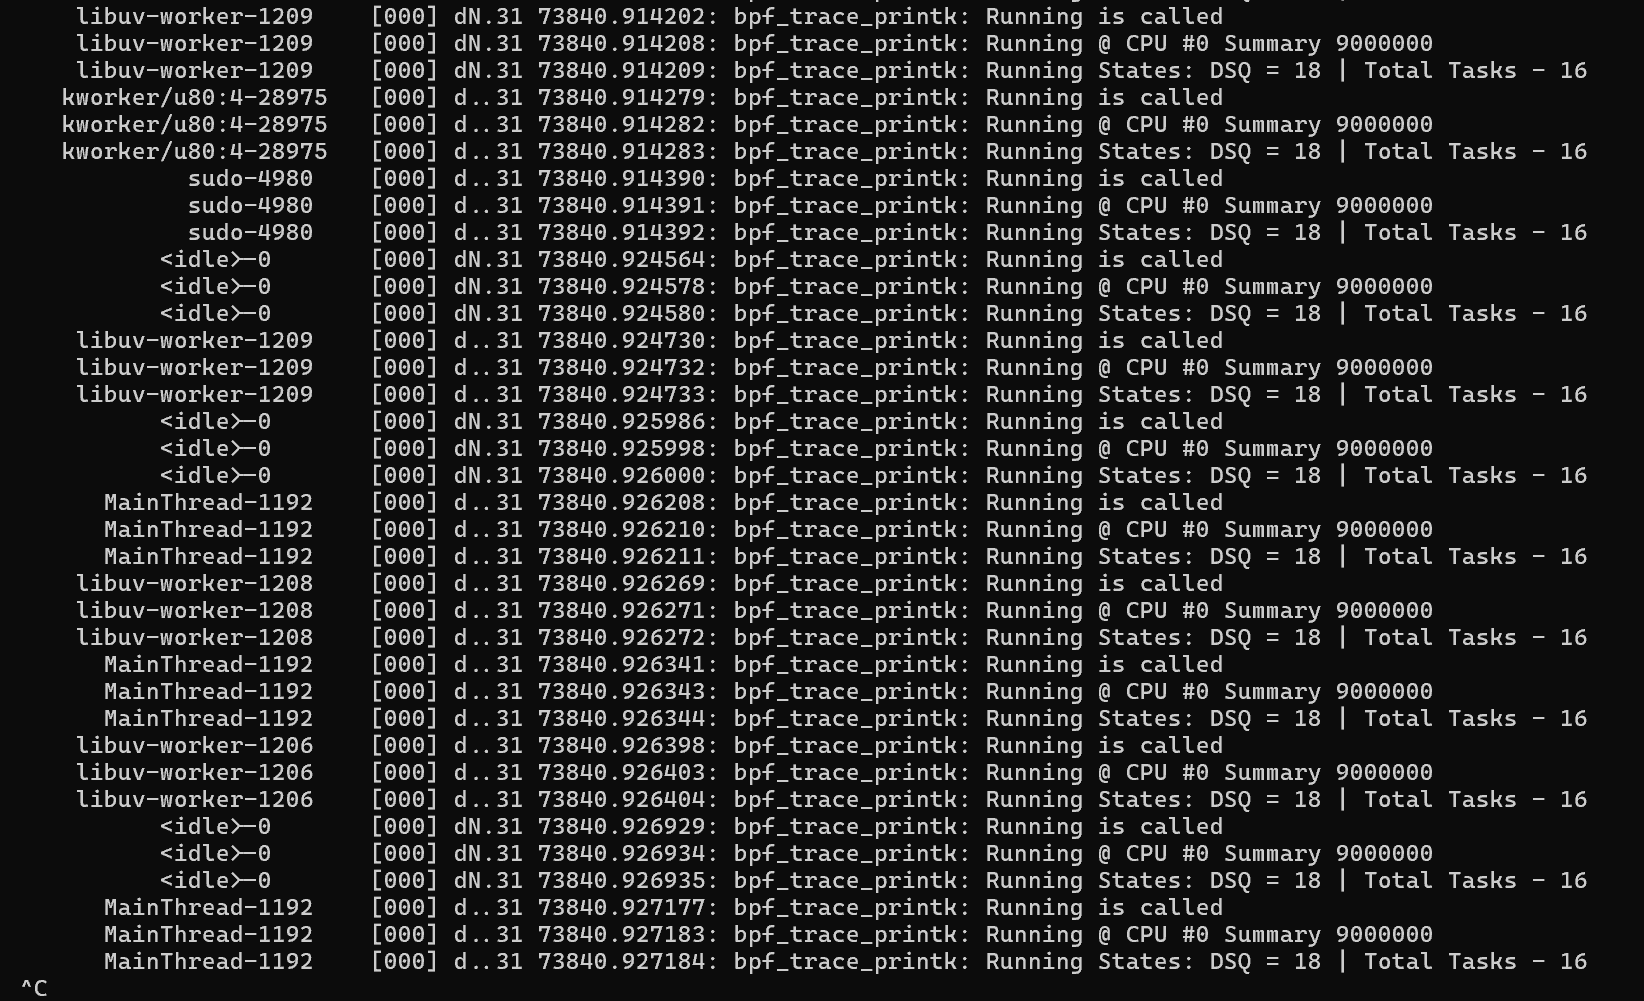
\includegraphics[width=22em]{logs.png}
  \end{center}
  \captionsetup{font=scriptsize}
  \vspace{-10pt}
  \caption{\scriptsize\label{fig:logs} Logs from 
  \texttt{/sys/kernel/debug/tracing/trace\_pipe} for the grid scheduler.}
\end{figure}

I have also begun designing the systems to transfer information about the
state and actions performed by my scheduler to user-space so it can be
analyzed when I begin performance evaluations. I will be using an eBPF
map to transmit information such as the number of tasks on each CPU or
each DSQ to user-space for observation. Additionally, I will be using
an event system that will be sent to user-space via a circular queue.
These events will be saved in user-space as a log. Next, I can parse
through the log to understand the behavior and performance of my scheduler.
I have begun preliminary work on implementing this system which includes
defining the types of events I am interested in.

%-------------------------------------------------------------------------------
\section{Challenges}
%-------------------------------------------------------------------------------

The largest current challenge is implementing the scheduler core logic
correctly. The current implementation which does not account for latency
requirement has a serious bug where the summary bitmap becomes inconsistent
with the actual state of the dispatch queues. This eventually causes some tasks
to be lost and not tracked by my summary bitmap. Ultimately, this causes the
task to sit within the queue until the scheduler terminates due to the
eBPF watchdog detecting the stalled process. Determining the source of where this
inconsistency arises has been tricky. 

A second challenge which I expect to face during the implementation of the scheduler
is ensuring a correct behavior when I introduce concurrency. The load balancing
mechanism will require CPUs to access other CPUs' data involving the state of their
grid. The current implementation uses a per-CPU eBPF map, but this prevents a
cross-CPU sharing needed for the load balancer. Ensuring a correct implementation
may be tricky due to the inconsistent behavior exhibited by concurrency.

Another problem I am anticipating is the implementation of the code handling
the latency requirement described in Section~\ref{sec:latency}. While the
core scheduling logic should be simple and the eBPF handlers for the system
calls should be simple, the majority of the work will be on aggregating
a list of system calls which may put a process to sleep. This work may be
onerous, but I do expect that I may only need to target a small subset
of these system calls for the performance evaluations.

%-------------------------------------------------------------------------------
\section{Preliminary Results}
%-------------------------------------------------------------------------------

I have no functional preliminary results to show here. As stated before, the
current partial implementation faces a bug in which the summary bitmap becomes
inconsistent with the state of the dispatch queues in the grid. This issue
ultimately causes some tasks on the dispatch queues to be ``lost'' while the
tasks waits on the queue leading to the scheduler being terminated. 
Figure~\ref{fig:logs} shows logs of the current partial scheduler implementation.

%-------------------------------------------------------------------------------
\section{Remaining Work}
%-------------------------------------------------------------------------------

The first remaining work to be done is to complete the implementation of the
grid scheduler. This will involve discovering the underlying bug with the
current implementation causing the summary bitmap to become inconsistent.
After this, the load balancer will be implemented. This will require some
significant adjustments to the current code including moving from the per-CPU
storage of the grid metadata into global memory. Again, this will involve
careful development to ensure no data races can occur that corrupts this
essential metadata used in scheduling algorithm. Finally, the detection of
the latency requirements will be implemented. 

With the scheduler implementation completed, my next step will be to implement
the logging subsystem that will report statistics and events back to user-space
for analysis. This will help prepare the scheduler to allow me to record the
performance and behavior of the scheduler to be used in my analysis. This step
may come earlier as it may also be useful when debugging my scheduler. 

Next, I will begin performance evaluations by comparing the performance of my
scheduler to EEVDF under different workloads. The specific benchmarks, hackbench
and Schbench, I will be using is the same from the proposal. I will also be
developing the synthetic benchmarks to demonstrate the problem with EEVDF, and
to show how my scheduler addresses these concerns. 

%-------------------------------------------------------------------------------
\bibliographystyle{plain}
\bibliography{\jobname}

%%%%%%%%%%%%%%%%%%%%%%%%%%%%%%%%%%%%%%%%%%%%%%%%%%%%%%%%%%%%%%%%%%%%%%%%%%%%%%%%
\end{document}
%%%%%%%%%%%%%%%%%%%%%%%%%%%%%%%%%%%%%%%%%%%%%%%%%%%%%%%%%%%%%%%%%%%%%%%%%%%%%%%%

%%  LocalWords:  endnotes includegraphics fread ptr nobj noindent
%%  LocalWords:  pdflatex acks